\documentclass{beamer}
\usepackage{amsmath}
\usepackage{array}
\usepackage{multirow}
\usepackage{eurosym}
\usepackage{tikz}

\newenvironment{conditions}
  {\par\vspace{\abovedisplayskip}\noindent\begin{tabular}{>{$}l<{$} @{${}={}$} l}}
  {\end{tabular}\par\vspace{\belowdisplayskip}}

\beamertemplatenavigationsymbolsempty{}
\usetheme{Goettingen}
\setbeamertemplate{footline}[frame number]
\usecolortheme{sidebartab}

%\setbeameroption{show only notes} % Only notes
%\setbeameroption{show notes on second screen=right} % Both

\mode<presentation>
\title[LoRaWAN]{Evaluation of LoRa and LoRaWAN with the Arduino boards and gateway}
\author{Oleg Bilovus}
\institute{Università degli Studi di Salerno}
\date[Lab of IoT 24/25]{Lab of IoT 2024/25}

\begin{document}
\begin{frame}
    \titlepage{}
    \note{We will talk about LoRa, LoRaWAN, the arduino boards which support the protocols and their gateway.}
\end{frame}

\AtBeginSection[]{
    \begin{frame}
        \frametitle{Outline}
        \tableofcontents[currentsection,subsubsectionstyle=hide]
    \end{frame}
}
\section{Background}
\begin{frame}
    \frametitle{Background}
    \begin{itemize}[<+->]
        \item \emph{Historically}, the Internet of Things (IoT) has been a fragmented market with a variety of technologies and standards.
        \item There are many protocols for IoT, but the most popular are Zigbee, Z-Wave,
              Bluetooth, Wi-Fi, and LoRaWAN\@.
        \item LoRaWAN is a low-power wide-area network (LPWAN) protocol based on the LoRa
              technology.
    \end{itemize}
\end{frame}

\subsection{LoRa}
\begin{frame}
    \frametitle{LoRa}
    \begin{itemize}[<+->]
        \item LoRa is a proprietary wireless communication technology developed by Semtech.
        \item It is a long-range, low-power, and low-bitrate technology.
        \item Data can be transmitted at a longer range compared to technologies like WiFi,
              Bluetooth or ZigBee.
        \item LoRa uses license-free sub-gigahertz radio frequency bands like 433 MHz, 868
              MHz (Europe), 915 MHz (USA), and 923 MHz (Asia).
        \item LoRa is ideal for applications that transmit small chunks of data with low bit
              rates.
    \end{itemize}
\end{frame}

\begin{frame}
    \frametitle{LoRa bandwidth vs range}
    \begin{figure}
        \centering
        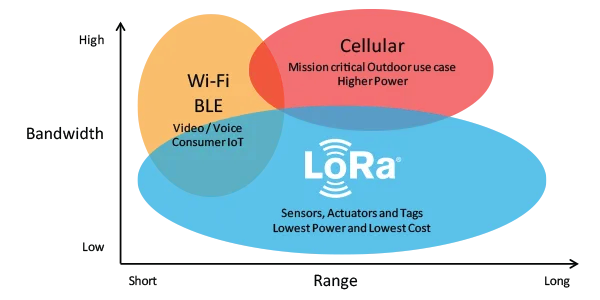
\includegraphics[width=\textwidth]{images/bandwidth-vs-range.png}
        \caption{LoRa bandwidth vs range}
    \end{figure}
\end{frame}

\subsection{LoRaWAN}
\begin{frame}
    \frametitle{LoRaWAN}
    \begin{itemize}[<+->]
        \item LoRaWAN is a Media Access Control (MAC) layer protocol built on top of LoRa
              modulation.
        \item It defines device communication and message formats using LoRa hardware.
        \item It is designed to support \emph{secure}, bi-directional communication,
              mobility, and localization services.
        \item LoRaWAN is optimized for low power consumption and supports large networks with
              millions of devices.
    \end{itemize}
\end{frame}

\begin{frame}
    \frametitle{LoRaWAN stack}
    \begin{figure}
        \centering
        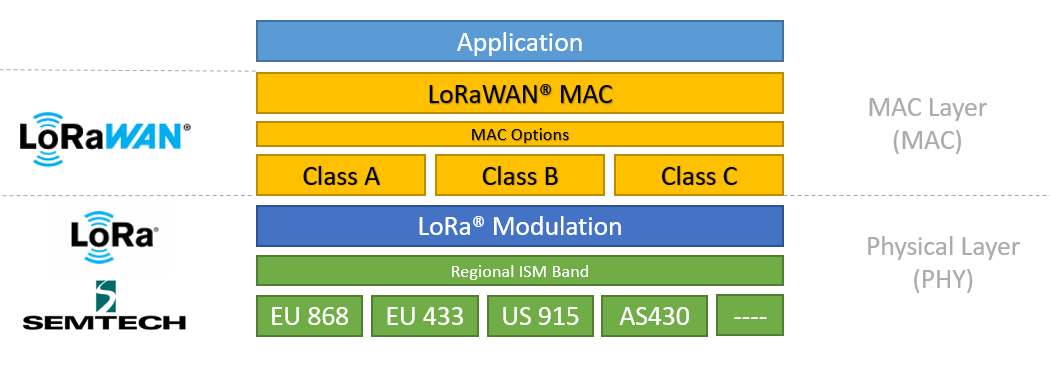
\includegraphics[width=\textwidth]{images/lorawan-stack.png}
        \caption{LoRaWAN protocol stack}
    \end{figure}
\end{frame}

\begin{frame}
    \frametitle{LoRaWAN architecture}
    \begin{figure}
        \centering
        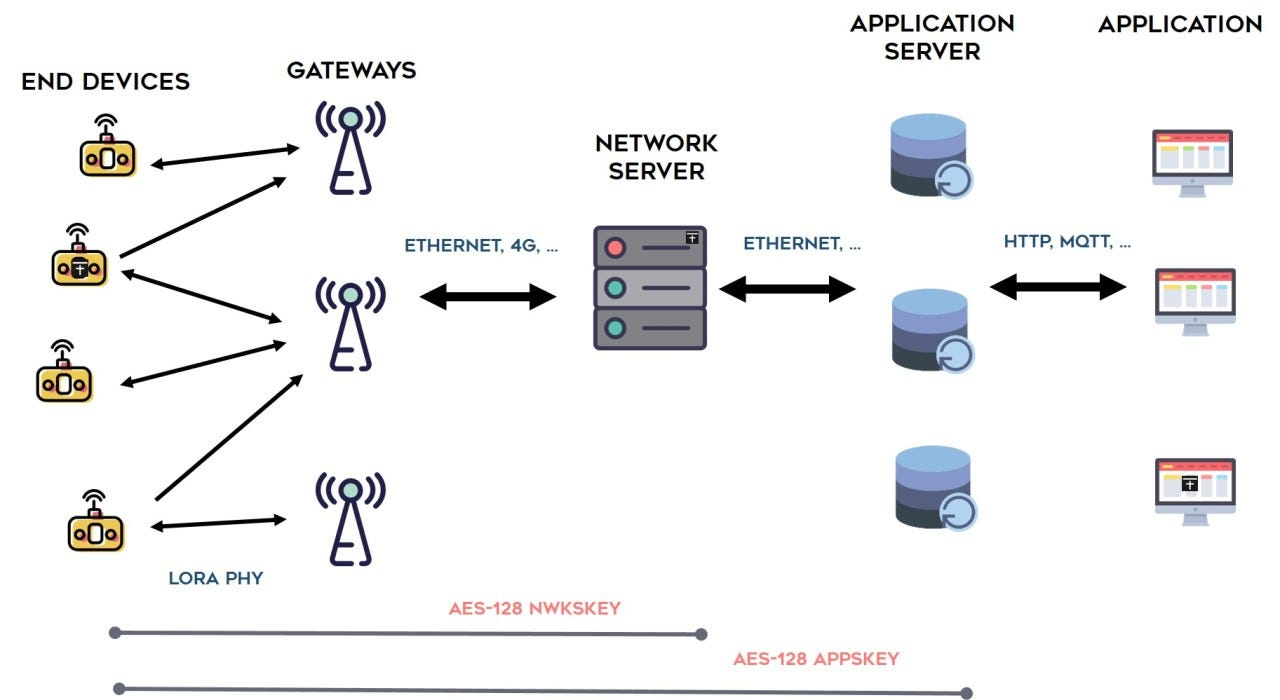
\includegraphics[width=\textwidth]{images/lorawan-architecture.jpg}
        \caption{LoRaWAN architecture}
    \end{figure}
\end{frame}

\section{Arduino}
\begin{frame}
    \frametitle{Arduino}
    \begin{itemize}[<+->]
        \item Arduino offers two main boards for the consumers that support LoRa and
              LoRaWAN\@: the MKR WAN 1300 and the MKR WAN 1310.
        \item Arduino offers two LoRaWAN gateway built by RAKwireless: one for indoor and one
              for outdoor use.
    \end{itemize}
\end{frame}
\subsection{Boards}
\begin{frame}
    \frametitle{Boards}
    \begin{columns}[]
        \begin{column}{0.5\textwidth}
            \begin{figure}
                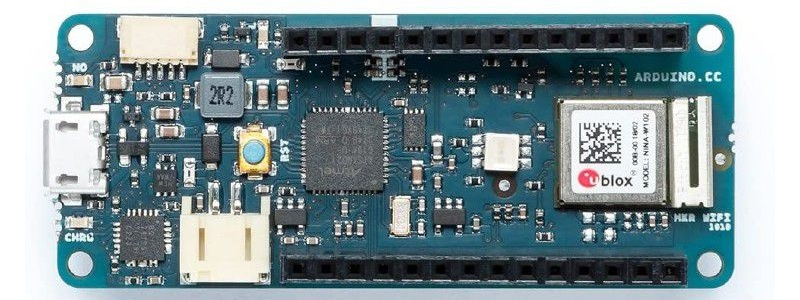
\includegraphics[width=\textwidth]{images/mkr1300.jpg}
                \caption{Arduino MKR WAN 1300}
            \end{figure}
        \end{column}
        \begin{column}<+->{0.5\textwidth}
            \begin{figure}
                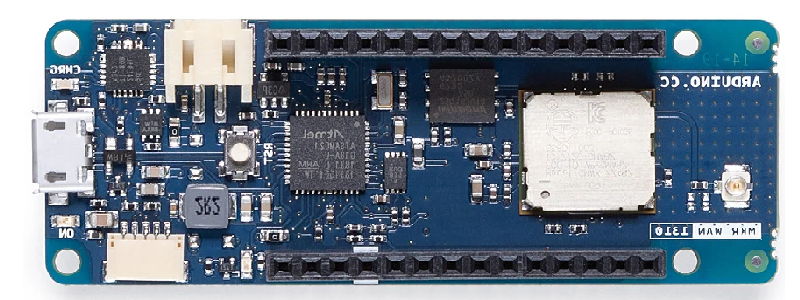
\includegraphics[width=\textwidth]{images/mkr1310.png}
                \caption{Arduino MKR WAN 1310}
            \end{figure}
        \end{column}
    \end{columns}

    \vspace{0.5cm}

    \begin{itemize}[<+->]
        \item The 1310 is an upgrade of the 1300.
        \item The main improvement is the energy consumption. The 1300 had a hardware design
              which resulted in an unnecessary high power consumption.
        \item The 1310 now also supports OTA (Over-The-Air) updates and data logging.
        \item The price is 50\euro.
    \end{itemize}
\end{frame}

\subsection{Gateway}
\begin{frame}
    \frametitle{Gateway}
    \begin{columns}[]
        \begin{column}{0.5\textwidth}
            \begin{figure}
                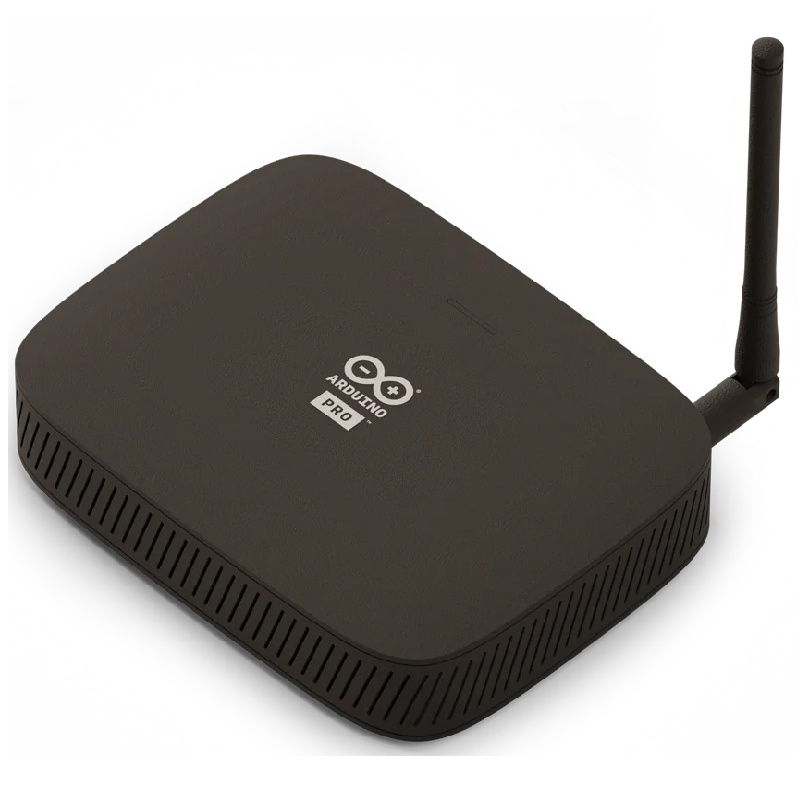
\includegraphics[width=\textwidth]{images/wisgate_indoor.png}
                \caption{WisGate Edge Lite 2 LoRaWAN indoor gateway}
            \end{figure}
        \end{column}
        \begin{column}<+->{0.5\textwidth}
            \begin{figure}
                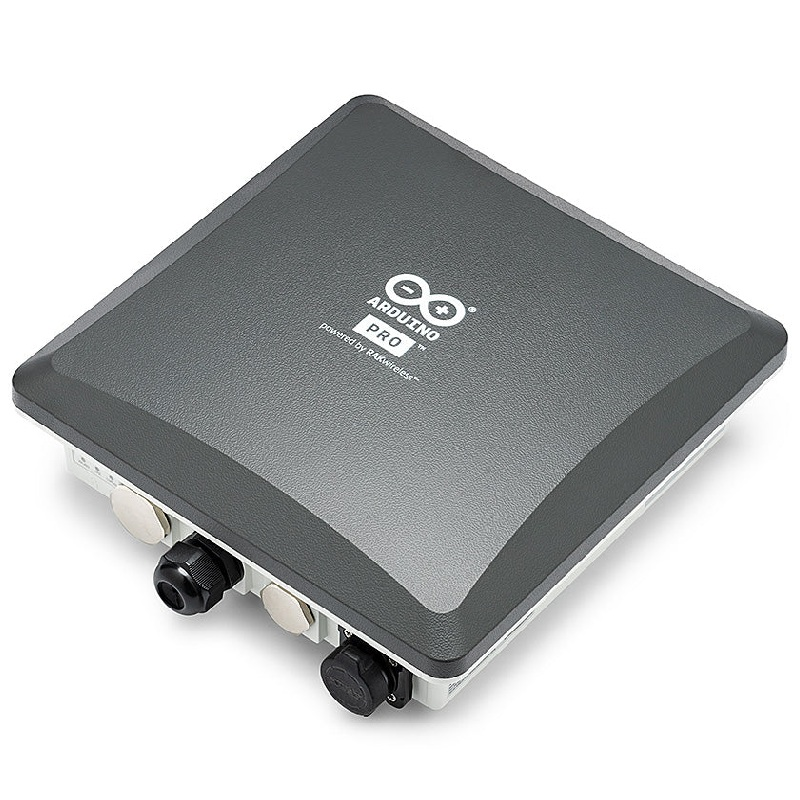
\includegraphics[width=\textwidth]{images/wisgate_outdoor.jpg}
                \caption{WisGate Edge PRO LoRaWAN outdoor gateway}
            \end{figure}
        \end{column}
    \end{columns}

    \vspace{0.5cm}

    \begin{itemize}[<+->]
        \item The outdoor gateway is a more professional device.
        \item The price is 270\euro{} for the indoor and 690\euro{} for the outdoor.
    \end{itemize}
\end{frame}

\section{Evaluation}

\subsection{LoRa}
\begin{frame}
    \frametitle{LoRa}
    \begin{itemize}[<+->]
        \item The LoRa technology is easy to use with the Arduino boards.
        \item It is not suitable for applications that require high data rates.
        \item It is not suitable for applications that require high reliability because there
              is no acknowledgment mechanism.
        \item It is not suitable for applications that require high security because the data
              is not encrypted.
        \item You can build your own protocol on top of LoRa.
    \end{itemize}
\end{frame}

\subsubsection{Gossiping}
\begin{frame}
    \frametitle{LoRa Gossiping}

    \begin{itemize}[<+->]
        \item A simple implementation of a gossiping protocol on top of LoRa where a node
              sends a message and the others forward it.
        \item The board with the blue LED sends a message.
        \item The boards with the white LED forward the message.
        \item If the message was already forwarded, the board with the white LED does not
              forward it again.
    \end{itemize}
\end{frame}

\begin{frame}
    \frametitle{LoRa Gossiping}
    \begin{center}
        Video of the LoRa gossiping
    \end{center}
\end{frame}

\subsection{LoRaWAN}
\begin{frame}
    \frametitle{LoRaWAN}
    \begin{itemize}[<+->]
        \item The LoRaWAN technology is easy to use with the Arduino boards thanks to the
              \emph{MKRWAN} library. But there is not much documentation and community
              support.
        \item It is suitable for applications that require high reliability because there is
              an acknowledgment mechanism.
        \item It is suitable for applications that require high security because the data is
              encrypted with AES 128.
    \end{itemize}
\end{frame}

\subsubsection{Multihop}
\begin{frame}
    \frametitle{LoRaWAN Multihop}
    \begin{itemize}[<+->]
        \item There is no official support for multi-hop or communication between end
              devices.
        \item By LoRaWAN specifications, the end devices can only communicate with the
              gateway.
        \item To build a multi-hop network, you need to use LoRa. But you will lose the
              acknowledgment mechanism and the security.
    \end{itemize}
\end{frame}

\begin{frame}
    \frametitle{LoRaWAN Multihop}
    In literature, there are some proposals to build a multi-hop network with LoRaWAN or a hybrid network with LoRa and LoRaWAN\@.
    But they are not official or widely used.
    \begin{figure}
        \centering
        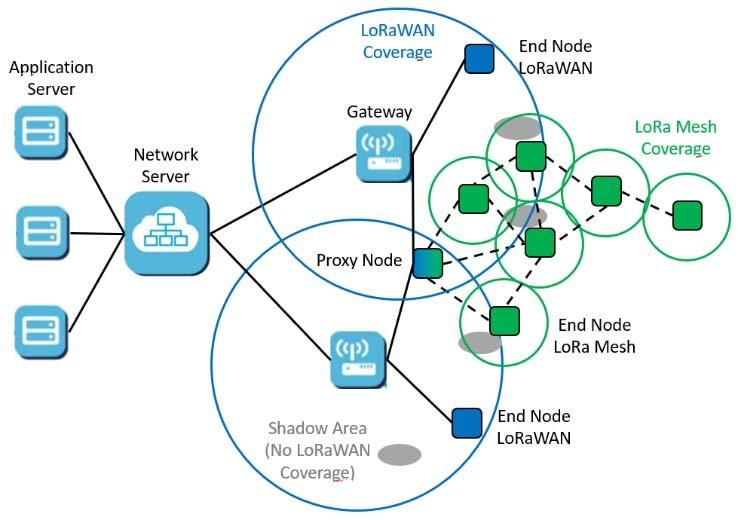
\includegraphics[width=0.8\textwidth]{images/lorawan_mesh.png}
        \caption{LoRaWAN hybrid network}
    \end{figure}
\end{frame}

\subsubsection{Project}
\begin{frame}
    \frametitle{LoRaWAN Project}
    \begin{itemize}[<+->]
        \item The project is to build a LoRaWAN network with the Arduino boards and the
              gateway.
        \item The boards will send their sensor data to the gateway.
        \item The gateway will send the data to a MQTT broker.
        \item The data will be extracted from the MQTT broker, decoded from base64, and sent
              to ThingsBoard and IoTPanels for the visualization. This is done with a GO
              script.
    \end{itemize}
\end{frame}

\begin{frame}
    \frametitle{LoRaWAN Project}
    \begin{columns}
        \begin{column}{0.5\textwidth}
            \begin{figure}
                \centering
                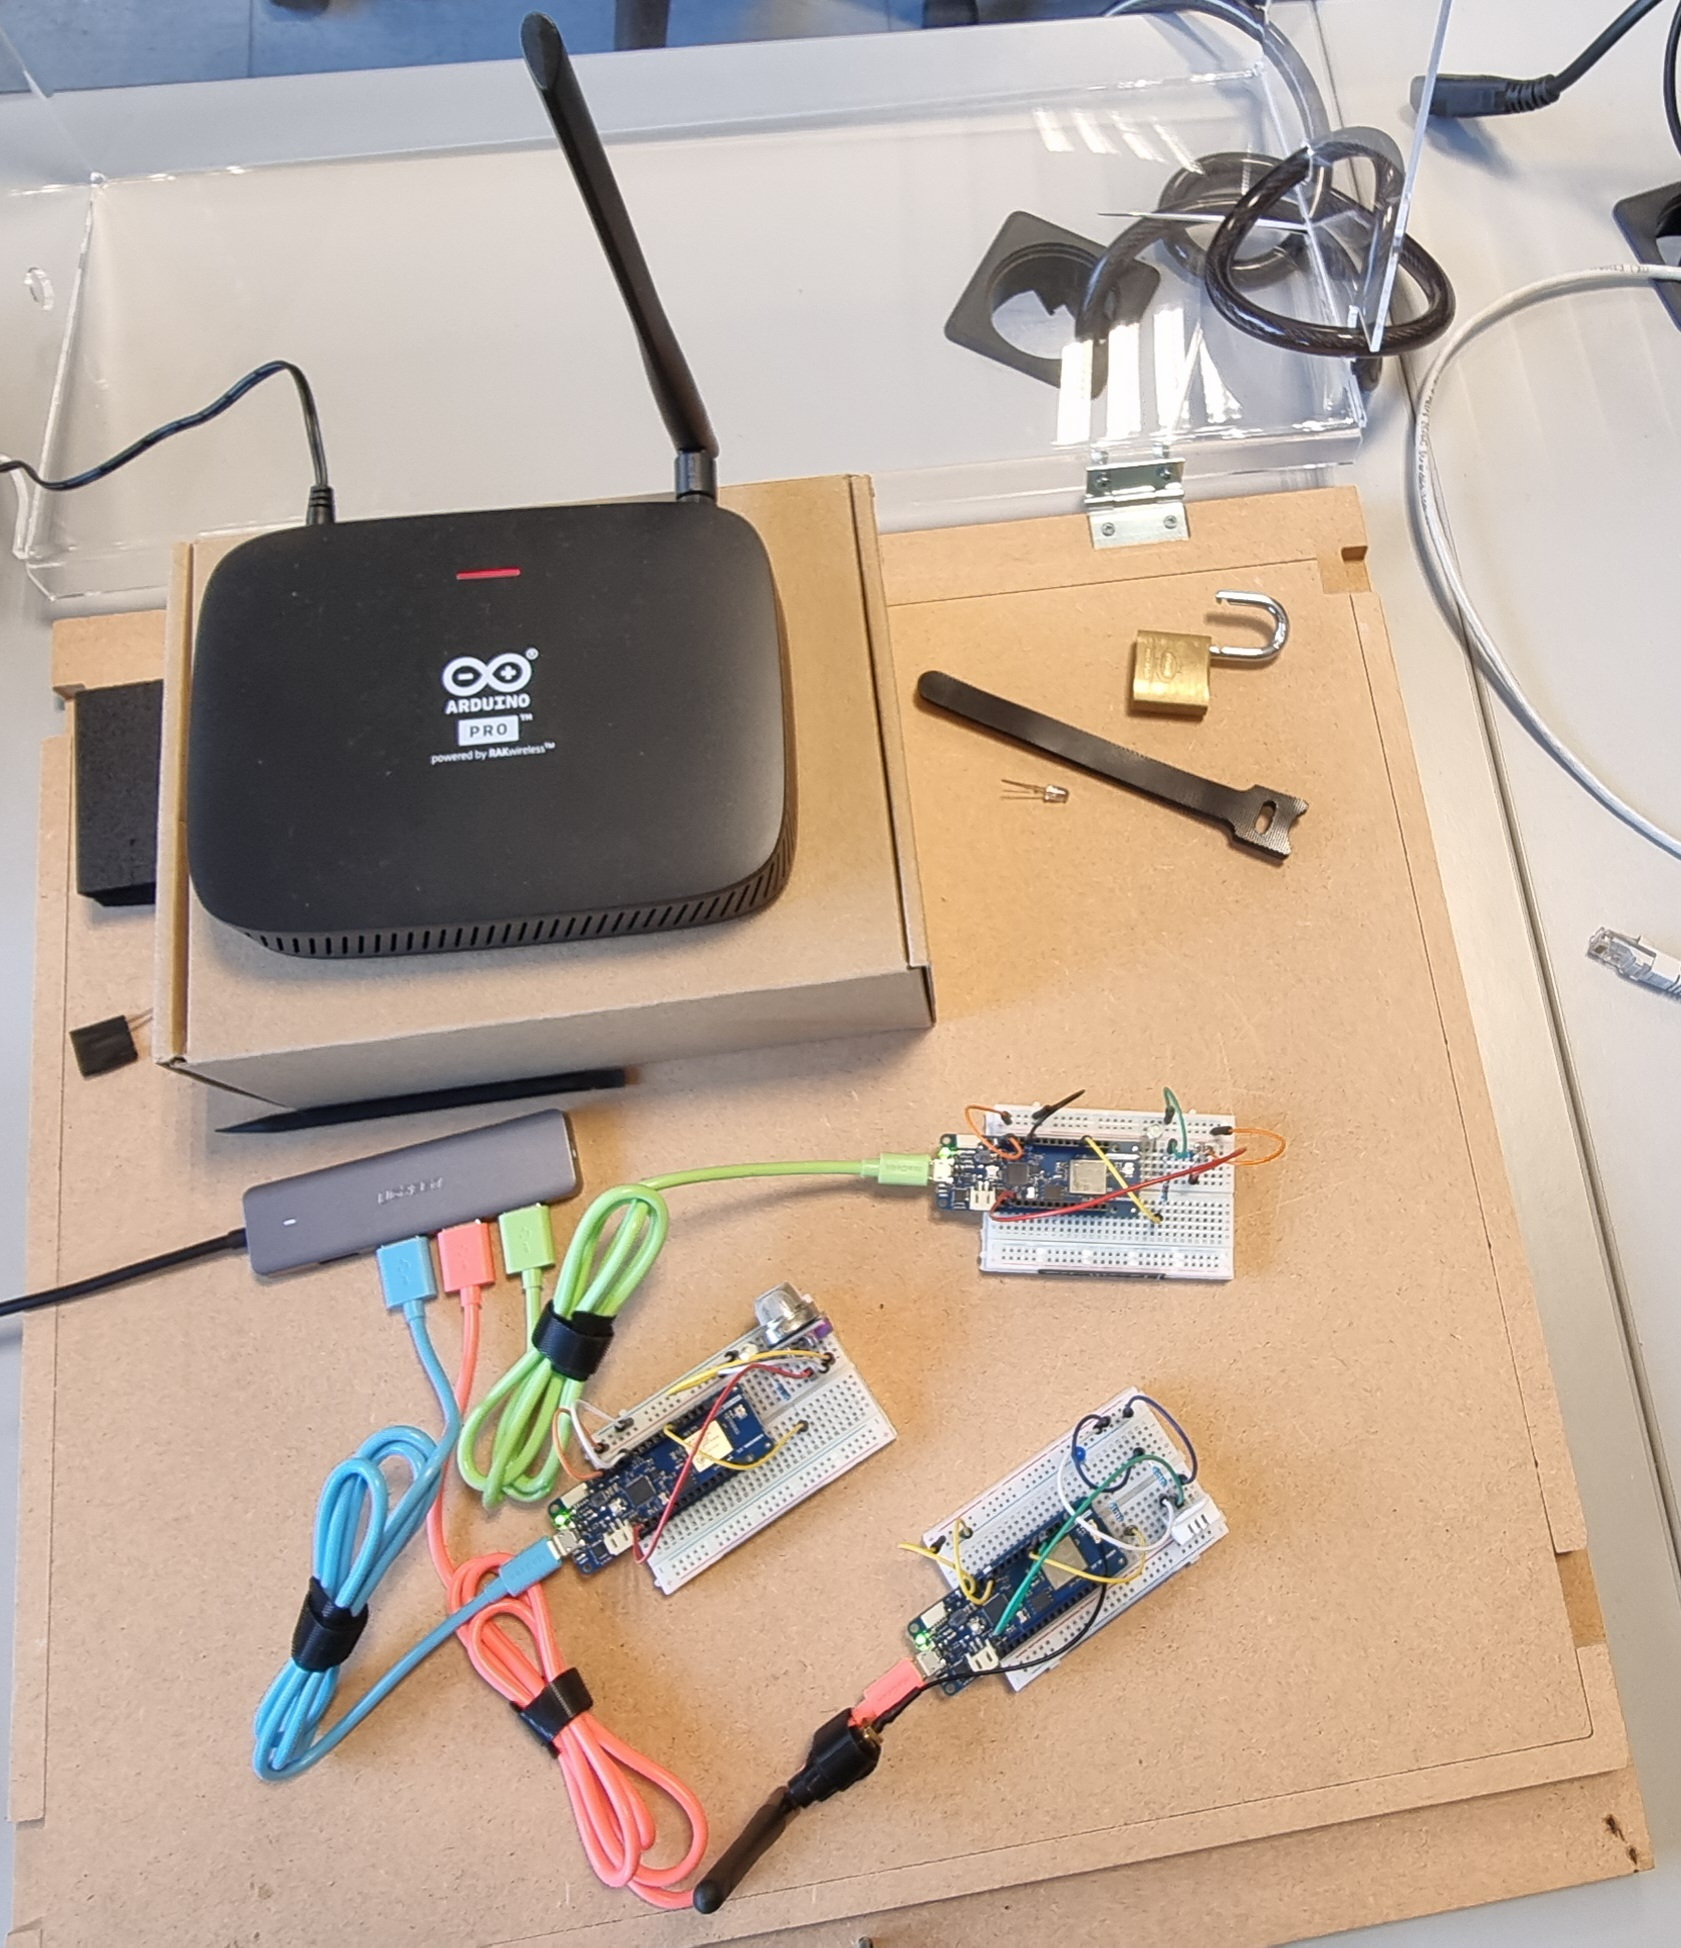
\includegraphics[width=\textwidth]{images/lorawan_project.jpg}
                \caption{LoRaWAN project}
                \begin{tikzpicture}[overlay, remember picture]
                    \node (board_dht11) at (0.8,2.5) {};
                    \node (board_light) at (0.8,3.5) {};
                    \node (board_mq2) at (-0.1,3) {};
                \end{tikzpicture}
            \end{figure}
        \end{column}
        \begin{column}{0.5\textwidth}
            \begin{itemize}[<+->]
                \item 3 Arduino MKR WAN 1310 boards.
                      \begin{itemize}[<+->]
                          \item \begin{tikzpicture}[overlay, remember picture]
                                    \draw[red, thick] (board_dht11) -- (-0.4,0.15);
                                \end{tikzpicture}
                                a board with a DHT22 sensor to measure the temperature and humidity.
                          \item \begin{tikzpicture}[overlay, remember picture]
                                    \draw[blue, thick] (board_mq2) -- (-0.4,0.15);
                                \end{tikzpicture}
                                a board with a MQ-2 sensor to measure the air quality.
                          \item \begin{tikzpicture}[overlay, remember picture]
                                    \draw[green, thick] (board_light) -- (-0.4,0.15);
                                \end{tikzpicture}
                                a board with a photoresistor to measure the light intensity.
                      \end{itemize}
            \end{itemize}
        \end{column}
    \end{columns}
\end{frame}

\begin{frame}
    \frametitle{LoRaWAN Project – ThingsBoard}
    \begin{figure}
        \centering
        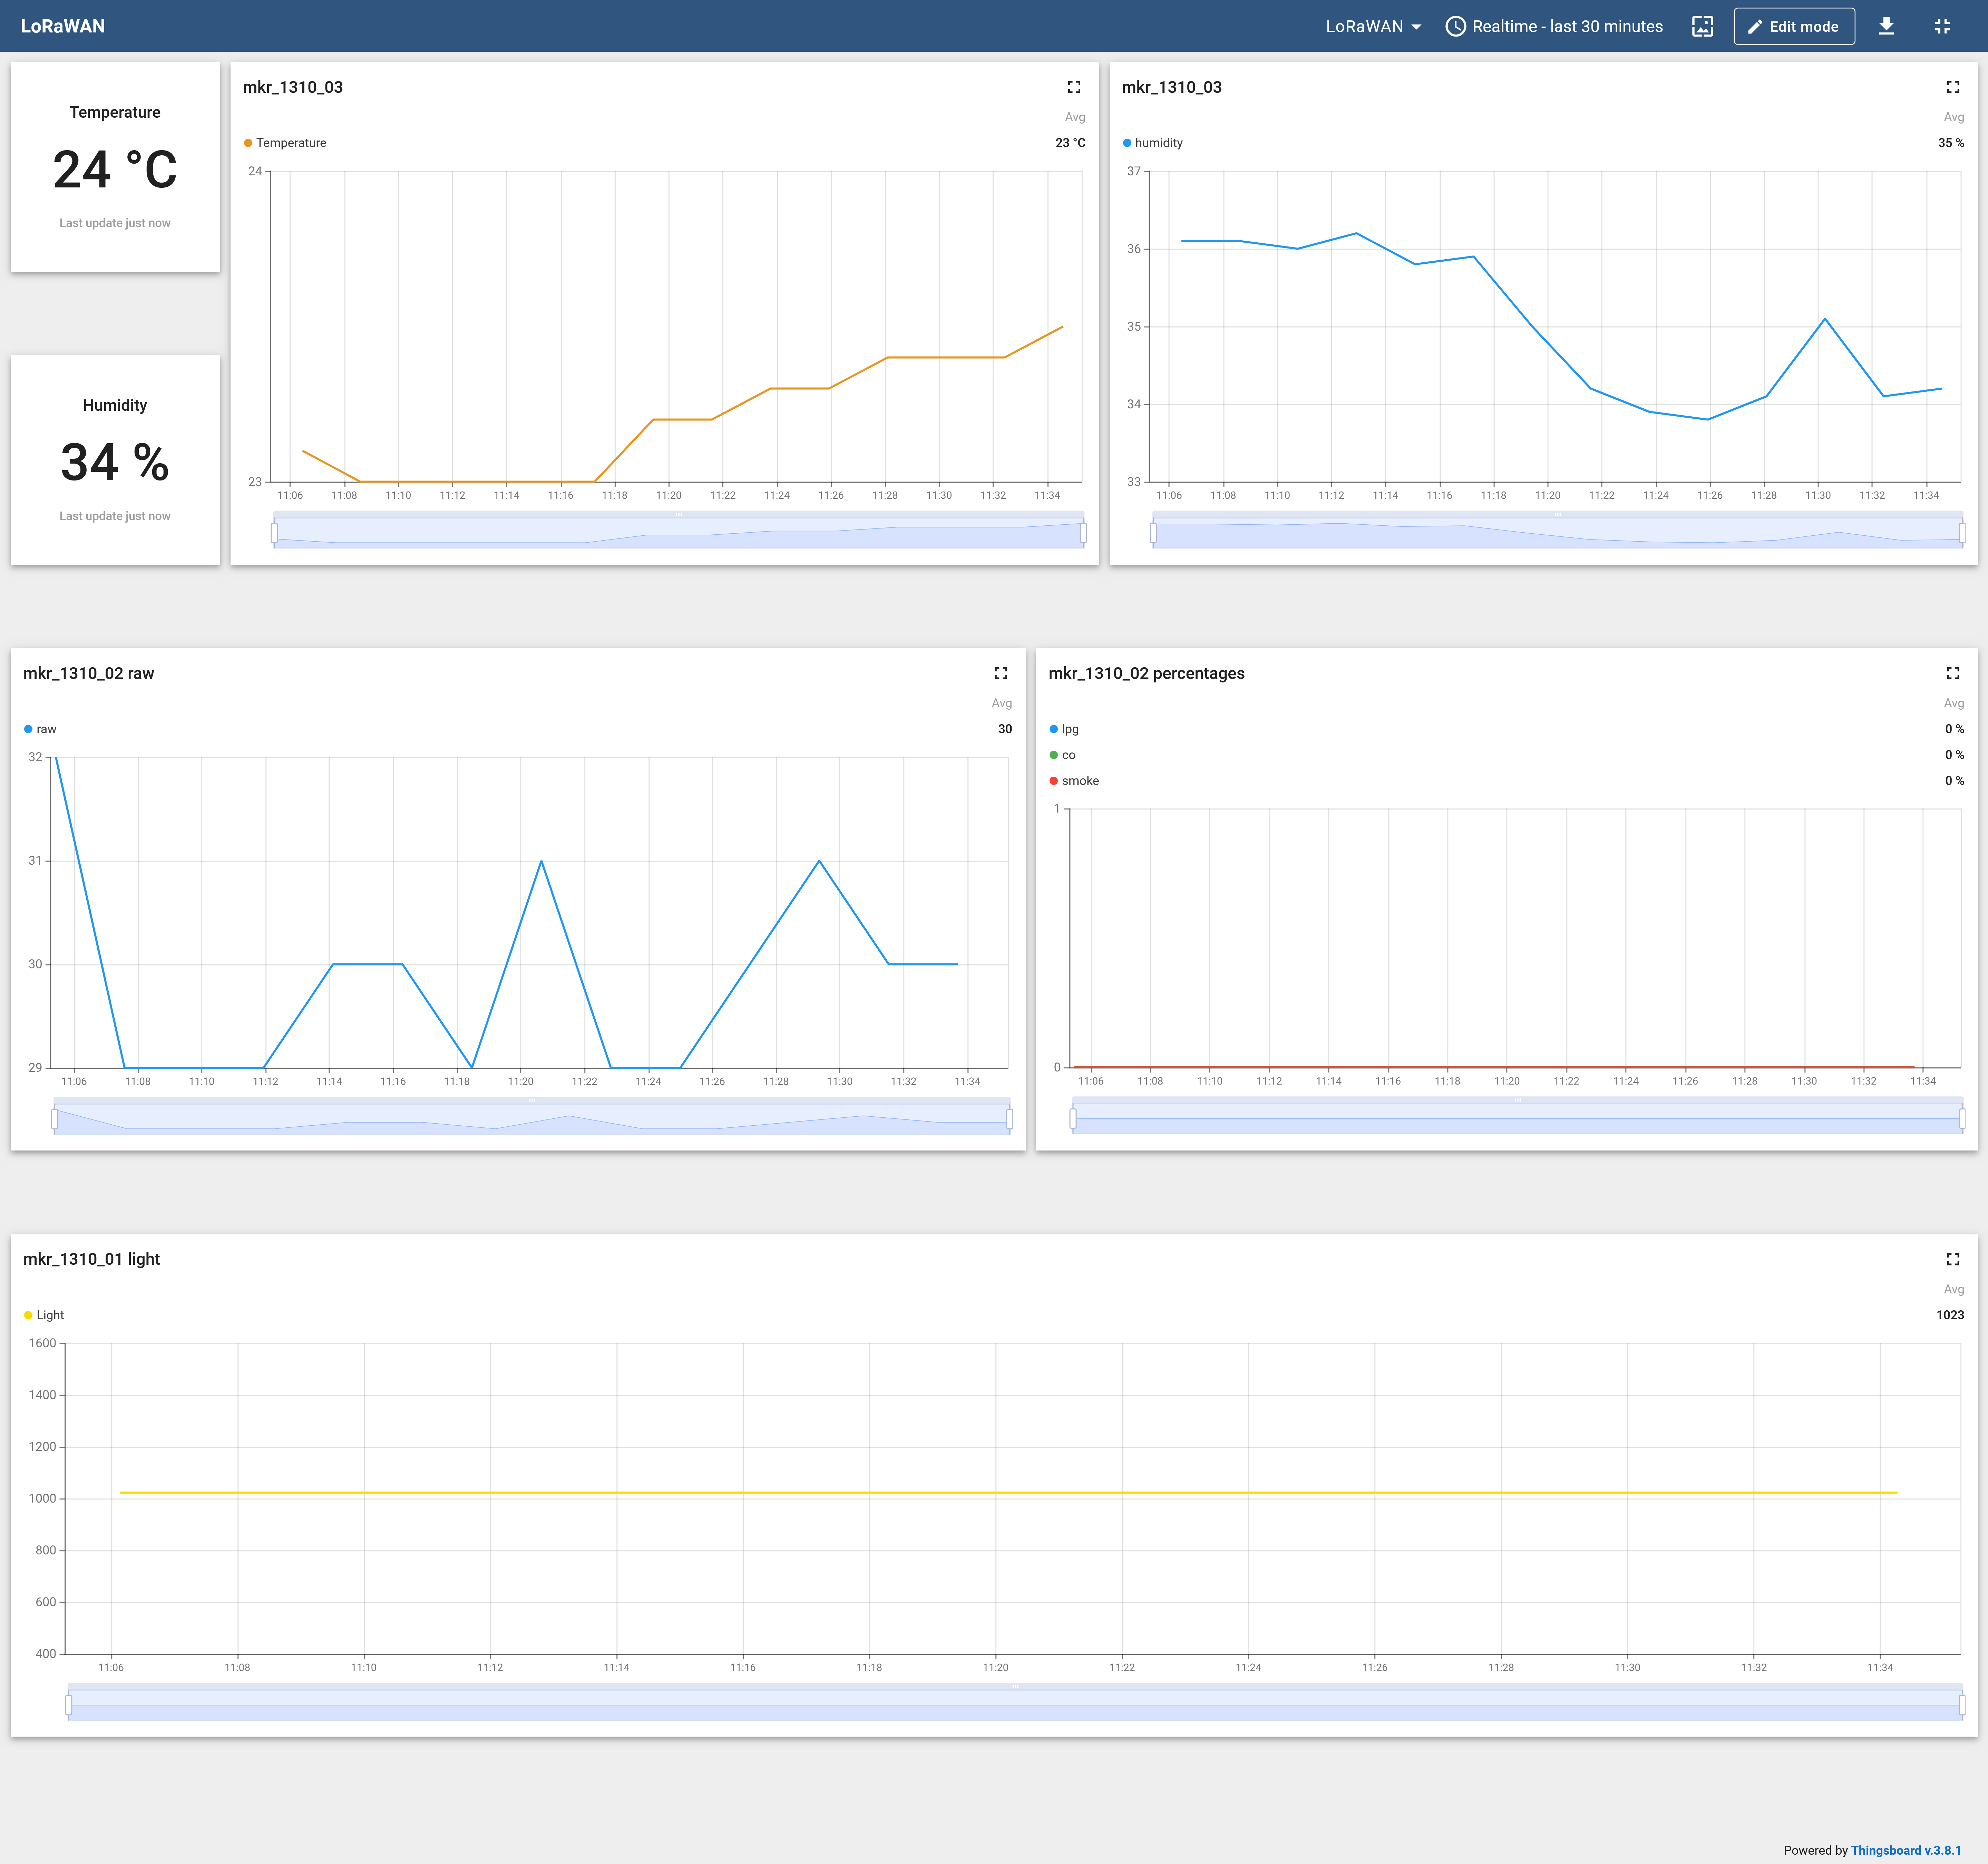
\includegraphics[width=\textwidth]{images/thingsboard.png}
        \caption{ThingsBoard}
    \end{figure}
\end{frame}

\begin{frame}
    \frametitle{LoRaWAN Project – IoTPanels}
    \begin{columns}
        \begin{column}{0.5\textwidth}
            \begin{figure}
                \centering
                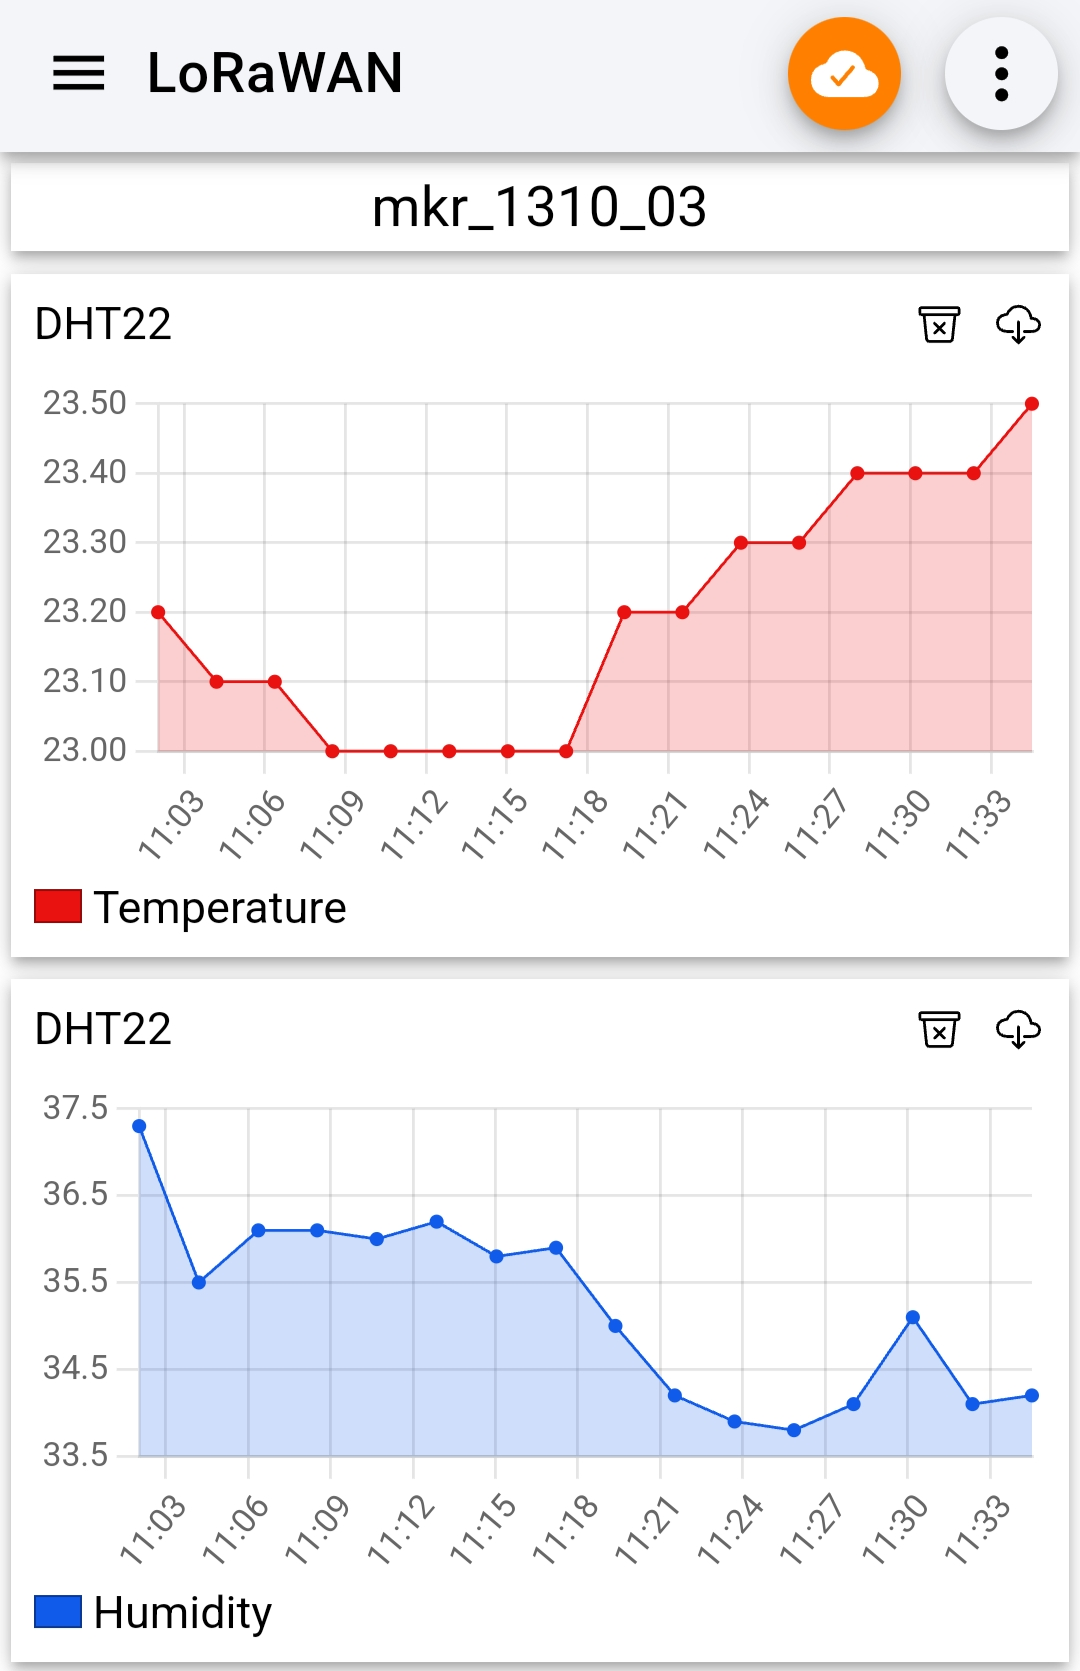
\includegraphics[width=\textwidth]{images/iotpanel_1.png}
            \end{figure}
        \end{column}
        \begin{column}{0.5\textwidth}
            \begin{figure}
                \centering
                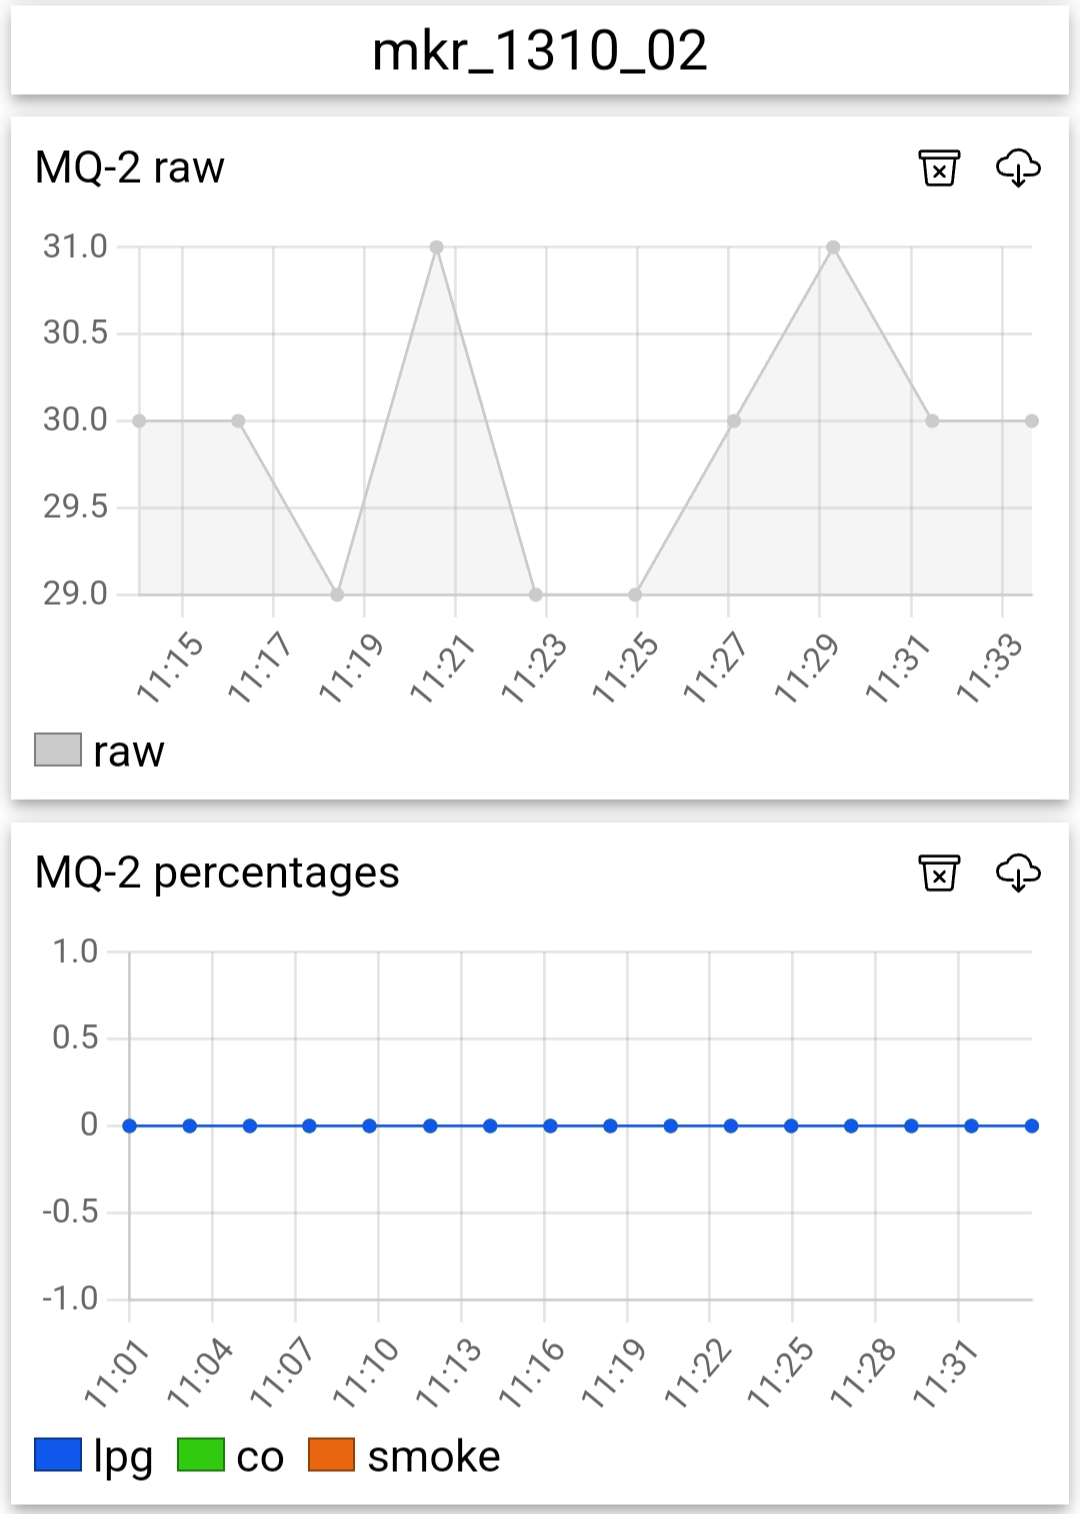
\includegraphics[width=\textwidth]{images/iotpanel_2.png}
            \end{figure}
        \end{column}
    \end{columns}
\end{frame}

\begin{frame}
    \frametitle{LoRaWAN Project – IoTPanels}
    \begin{columns}
        \begin{column}{0.5\textwidth}
            \begin{figure}
                \centering
                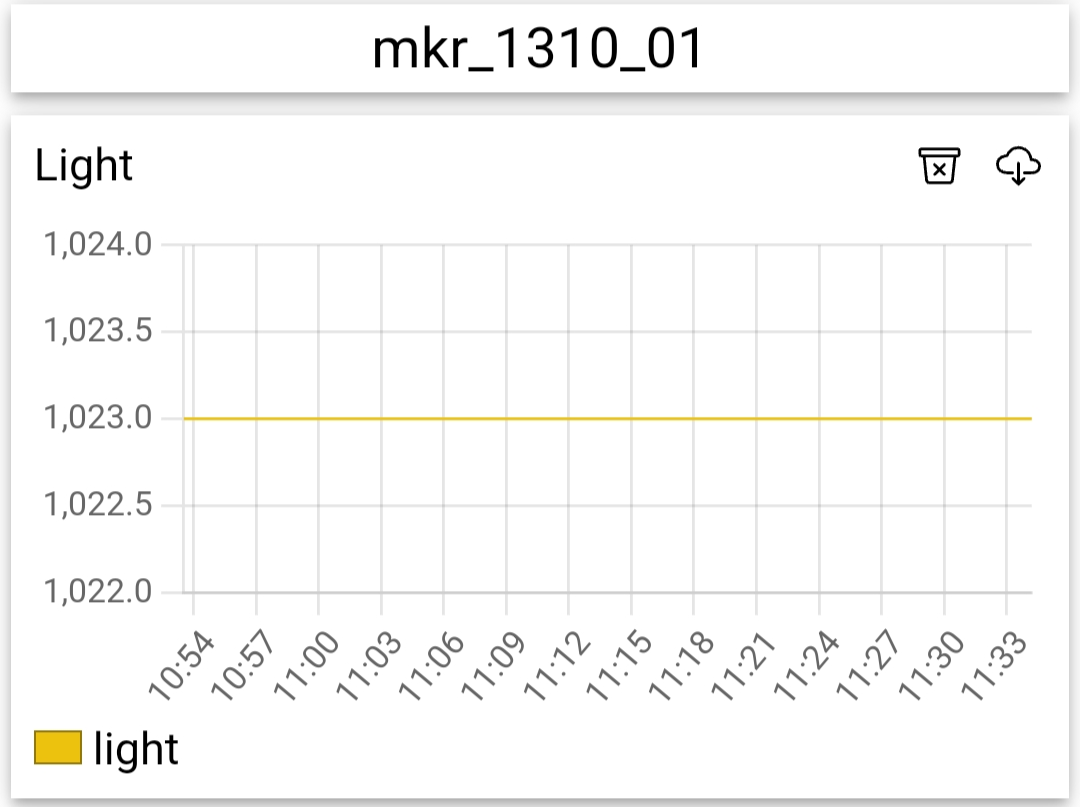
\includegraphics[width=\textwidth]{images/iotpanel_3.png}
            \end{figure}
        \end{column}
        \begin{column}{0.5\textwidth}
            \begin{figure}
                \centering
                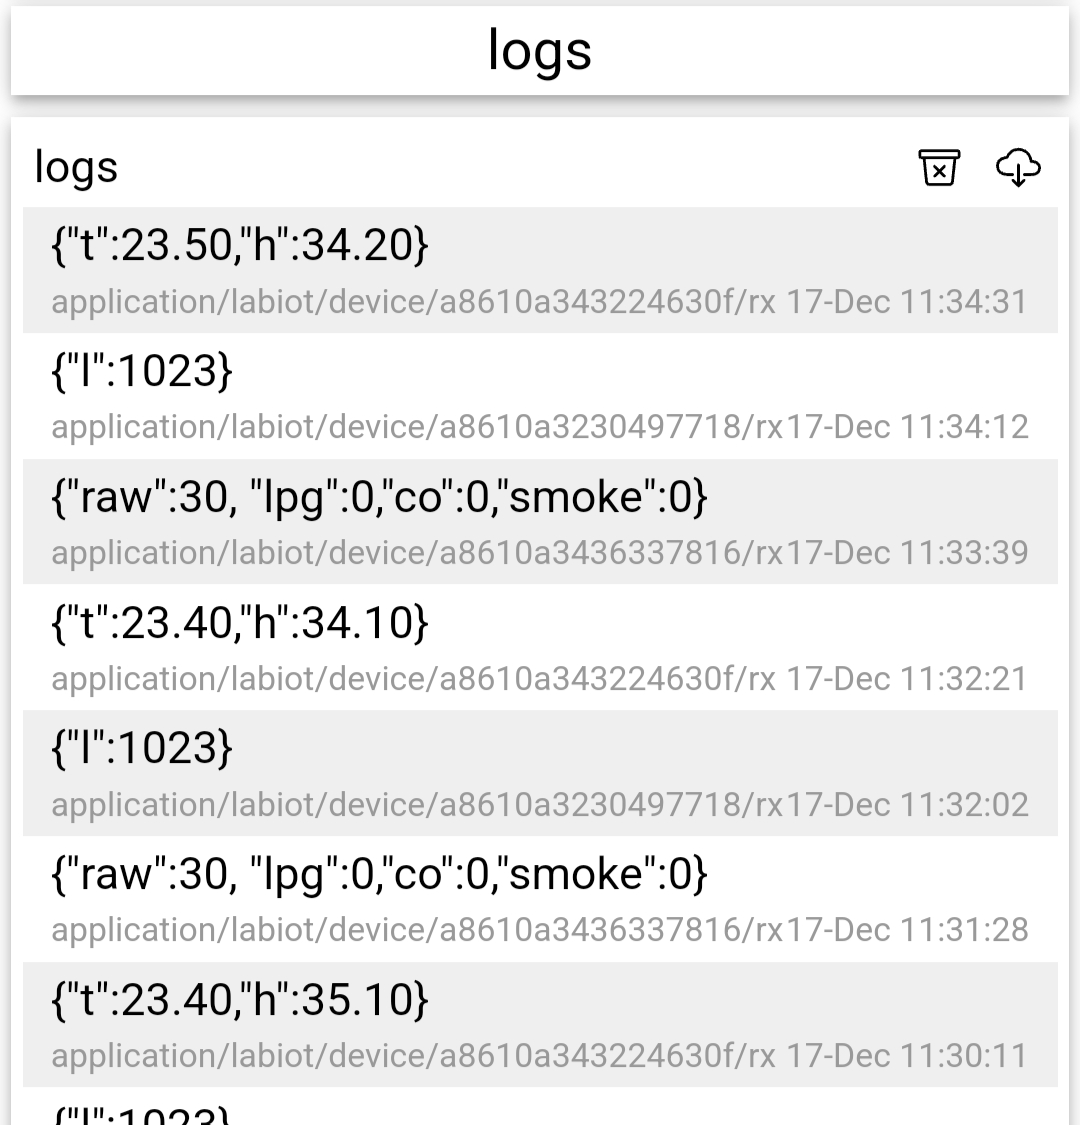
\includegraphics[width=\textwidth]{images/iotpanel_4.png}
            \end{figure}
        \end{column}
    \end{columns}
\end{frame}

\subsection{Boards}
\begin{frame}
    \frametitle{Boards}
    \begin{itemize}[<+->]
        \item The Arduino boards are easy to use with the LoRa and LoRaWAN technologies.
        \item The documentation and community support are not very good because these boards
              seems not to be widely used. Probably because people prefer to use a LoRa
              module and a microcontroller separately.
        \item The 1300 version has a high power consumption and some software/hardware issues
              when uploading the sketch.
        \item The boards are probably not suitable for professional applications, but they
              are good for educational purposes or home projects.
    \end{itemize}
\end{frame}

\begin{frame}
    \frametitle{Boards}
    \begin{itemize}[<+->]
        \item The transmission range indoor was not very good. In a university building with
              concrete walls, the range was about 100 meters.
        \item You can transmit data to the gateway every 2 minutes. This is enforced by the
              board firmware and it is not a limitation of the LoRaWAN technology.
        \item You can not use use both LoRa and LoRaWAN at the same time because their
              configuration conflicts.
    \end{itemize}
\end{frame}

\subsection{Gateway}
\begin{frame}
    \frametitle{Gateway}
    \begin{itemize}[<+->]
        \item The first setup of the gateway is not easy because there are missing
              informations in the documentation. For example, the gateway needs 10–15 minutes
              to boot up and this is written nowhere.
        \item Updating the firmware may corrupt some settings and you need to set them again.
              In the UI, it will show as they are set, but they are not.
        \item You can only have 1 tab open in the UI\@. If you open a second tab, the first
              one will be disconnected. This means multiple users can not use the UI at the
              same time.
        \item You have to go to the RAKwireless documentation to find most of the
              informations.
        \item Overall, the main issue is the missing of a detailed documentation by Arduino
              and RAKwireless. There is also a very poor community support because the
              gateway is not widely used.
    \end{itemize}
\end{frame}

\section{Conclusion}
\begin{frame}
    \frametitle{Conclusion}
    \begin{itemize}[<+->]
        \item LoRa and LoRaWAN are good technologies for IoT applications that require low
              power consumption and long-range communication.
        \item The Arduino boards are easy to use with the LoRa and LoRaWAN technologies, but
              the documentation and community support are not very good.
        \item The Arduino boards are probably not suitable for professional applications, but
              they are good for educational purposes or home projects.
        \item The gateway is not easy to set up because of the missing informations in the
              documentation and the poor community support.
        \item The tested transmission range indoor was not very good.
    \end{itemize}
\end{frame}

\begin{frame}
    \nocite{*}
    \frametitle{References}
    \bibliographystyle{amsalpha}
    \bibliography{bib.bib}
\end{frame}
\end{document}